\documentclass[12pt]{article}

% фонтови и језик
% fontspec docs: shorturl.at/ouI26
\usepackage{fontspec}

% polyglossia docs: shorturl.at/gELX9
\usepackage{polyglossia}
\newfontfamily\cyrillicfont{Times New Roman} % може се заменити компатибилним фонтом
\newfontfamily\cyrillicfontsf{Arial}         % може се заменити компатибилним фонтом
\newfontfamily\cyrillicfonttt{Courier New}   % може се заменити компатибилним фонтом
\setmainlanguage[Script=cyrillic]{serbian}
\setotherlanguage{english}

% вербатим линкови (веб адресе, имејлови, релативне адресе, итд.)
% url docs: shorturl.at/iktM4
\usepackage{url}

% хиперлинкови
% hyperref docs: shorturl.at/fmHPW
\usepackage{hyperref}

% приказивање математичких израза
% amsmath docs: shorturl.at/avJU3 
\usepackage{amsmath}

% напредни пакет за исцрватање графика коришћењем команде \includegraphics
% graphicx docs: shorturl.at/diHUW
\usepackage{graphicx}
\graphicspath{{images/}}    % коренски директоријум слика, сваки пут када се користи includegraphics команда путања која се задаје треба да буде релативна у односу на овај директоријум

% рад са прилозима
% appendix docs: shorturl.at/uwEL1
\usepackage{appendix}

% подешавања маргина
\usepackage{vmargin}
\setmarginsrb{3 cm}{2.5 cm}{3 cm}{2.5 cm}{1 cm}{1.5 cm}{1 cm}{1.5 cm}

% исцртавање програмског кода
\usepackage{minted}

% подешавање размака линија текста
\usepackage{setspace}

% цртање табела
\usepackage{booktabs}

% додатни макрои за израду рада
\usepackage{rsvp}


\title{Паралелизација проблема проналажења суме у бинарном стаблу}                         % ТОДО изменити
\author{Бојан Попржен}                  % ТОДО изменити
\newcommand{\studentindex}{E2 4/2022}     % ТОДО изменити

\usepackage{fancyhdr}

\makeatletter
\let\thetitle\@title
\let\theauthor\@author
\let\thedate\@date
\let\theindex\studentindex
\makeatother

\pagestyle{fancy}
\fancyhf{}
\rhead{\theauthor}
\lhead{\thetitle}
\cfoot{\thepage}


\begin{document}
\begin{titlepage}
	\centering
    \vspace*{0.5 cm}
    
\includegraphics[scale = 0.75]{ftn-logo.eps}\\[1.0 cm]	                % University Logo
    \textsc{\LARGE Факултет техничких наука}\\[0.5 cm]	                    % University Name
	\textsc{\Large Универзитет у Новом Саду}\\[1.0 cm]				        % Course Code
	\textsc{\large Рачунарски системи високих перформанси}\\[0.5 cm]		% Course Name
	\rule{\linewidth}{0.2 mm} \\[0.4 cm]
	{ \huge \bfseries \thetitle}\\
	\rule{\linewidth}{0.2 mm} \\[1.5 cm]
	
	\begin{minipage}{0.4\textwidth}
		\begin{flushleft} \large
			\emph{Аутор:}\\
			\theauthor
			\end{flushleft}
			\end{minipage}~
			\begin{minipage}{0.4\textwidth}
			\begin{flushright} \large
			\emph{Индекс:} \\
			\theindex								                        % Your Student Number
		\end{flushright}
	\end{minipage}\\[2.0 cm]
	
	{\large \thedate}\\[2 cm]
	\vfill
\end{titlepage}

\pagenumbering{roman}
\begin{abstract}
\doublespacing
У овом раду анализиран је проблем проналажења суме у бинарном стаблу.
Проблем проналажења суме у бинарном стаблу можемо представити питањем: "Да ли чворови бинарног стабла којима је придружен
природан број у било којој путањи од корена до листа дају задати збир?".
Поступак за решавање овог проблема могуће је разложити на независне делове које је могуће паралелно решити.
Решење проблема приказано у овом раду пружа приближно линеарно убрзање доласка до решења са порастом броја процесуирајућих јединица.
\end{abstract}
\pagebreak          % ТОДО попунити              
%%%%%%%%%%%%%%%%%%%%%%%%%%%%%%%%%%%%%%%%%%%%%%%%%%%%%%%%%%%%%%%%%%%%%%%%%%%%%%%%%%%%%%%%%

% садржај
\tableofcontents
\pagebreak

%%%%%%%%%%%%%%%%%%%%%%%%%%%%%%%%%%%%%%%%%%%%%%%%%%%%%%%%%%%%%%%%%%%%%%%%%%%%%%%%%%%%%%%%%

% листинг изворних кодова
\listoflistings
\pagebreak

%%%%%%%%%%%%%%%%%%%%%%%%%%%%%%%%%%%%%%%%%%%%%%%%%%%%%%%%%%%%%%%%%%%%%%%%%%%%%%%%%%%%%%%%%

% листинг фигура
\listoffigures
\pagebreak

%%%%%%%%%%%%%%%%%%%%%%%%%%%%%%%%%%%%%%%%%%%%%%%%%%%%%%%%%%%%%%%%%%%%%%%%%%%%%%%%%%%%%%%%%

% листинг табела
\listoftables
\pagebreak

%%%%%%%%%%%%%%%%%%%%%%%%%%%%%%%%%%%%%%%%%%%%%%%%%%%%%%%%%%%%%%%%%%%%%%%%%%%%%%%%%%%%%%%%%

\pagenumbering{arabic}
\section{Увод}
У овом раду, анализиран је проблем проналажења суме у бинарном стаблу. Проблем можемо представити и питањем: "Да ли чворови бинарног стабла којима је придружен
природан број у било којој путањи од корена до листа дају задати збир?".

Најчешће решење овог problema има асимптотску временску сложеност извршавања $O(n)$ gde $n$ представља величину улаза tj. број чворова у графу.

У овом раду, предложено је паралелно решење проблема које узима у обзир независност обраде деце одређеног чвора.

Постигнута асимптотска сложеност паралелног решења је приближно: $O(n/p)$, где је $n$ величина улаза тј. број чворова у графу, а $p$ број јединица паралелног извршавања.

Рад је конципиран на следећи начин: прво ће сам проблем бити описан као и његово секвенцијално решење, потом ће бити приказано паралелно решење и
, на крају, биће представљени подаци о ефикасности секвенцијалног и паралелног решења.
\pagebreak              % ТОДО попунити

\section{Проблем проналаска суме у бинарном стаблу}

\subsection{Опис проблема}
Cтабло је граф који је повезан и који нема циклуса.
Бинарно стабло је усмерено стабло у коме сваки чвор, почевши од коренског чвора, има 0, 1 или 2 деце-чворова. Дететом чвора називамо чвор на кога неки други чвор показује.
Родитељем чвора називамо чвор који на неки други чвор показује. Листом називамо чвор који има 0 деце.

\begin{figure}[H]
    \centering
    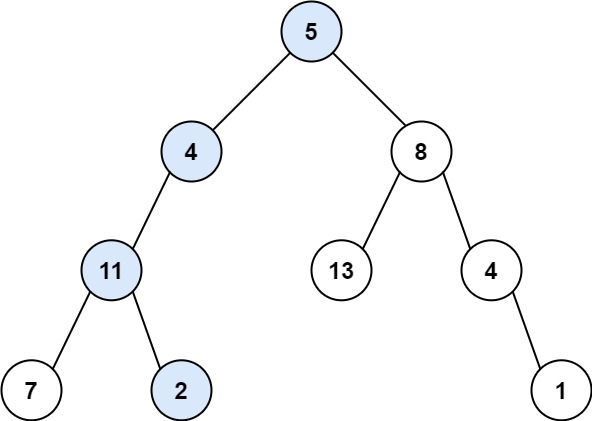
\includegraphics[scale = 0.4]{pathsum1.jpg}
    \caption{Пример постојања тражене путање за проблем проналаска суме у бинарном стаблу}
    \label{fig:primersume}
\end{figure}

У примеру \ref{fig:primersume}, плавом је приказана једна путања која даје тражену суму \textbf{22}.


\begin{table}[H]
    \centering
    \begin{tabular}{@{}c|c@{}}
        & \textbf{Улаз}           \\
        \hline
    1 & Бинарно стабло \\
    2 & Тражена сума  
    \end{tabular}
    \caption{Табела улаза за проблем проналаска суме у бинарном стаблу}
    \label{table:ulazi}
\end{table}

\begin{table}[H]
    \centering
    \begin{tabular}{@{}c|c@{}}
      & \textbf{Излаз}             \\
      \hline
    1 & Булова променљива
    \end{tabular}
    \caption{Табела излаза за проблем проналаска суме у бинарном стаблу}
    \label{table:izlazi}
\end{table}

За проблем су дата два улаза (табела \ref{table:ulazi}): стабло и тражена сума, док је тражен један излаз (табела \ref{table:izlazi}): булова променљива чија је тачност еквивалентна чињеници да је решење пронађено, односно
да за дати граф постоји путања од корена до листа која даје тражену суму.

\subsection{Секвенцијално решење проблема}

Најчешће секвенцијално решење проблема своди се на обилазак графа по дубини (енг. \textit{depth first search}, DFS).

Секвенцијално решење прво обради (по дубини) лево дете-чвор па потом десно.
Обрада појединачног чвора своди се на следећи поступак:

Постави тренутан чвор на УЛАЗ 1 (корен стабла). Постави тренутно тражену суму на УЛАЗ 2 (тражену суму).
Покрени обраду описану корацима:

\begin{enumerate}
    \item Уколико је тренутан чвор нула-чвор, врати НЕТАЧНО.
    \item Уколико тренутан чвор није нула-чвор:
    \begin{enumerate}
        \item Уколико је број придружен чвору већи од тренутно траженог збира, врати НЕТАЧНО.
        \item Уколико је број придружен чвору једнак тренутно траженом збиру и тренутни чвор је лист, врати ТАЧНО.
        \item Уколико је број придружен чвору мањи или једнак тренутно траженом збиру, умањи тренутно тражени збир за тај број. А потом:
        \begin{enumerate}
            \item Уколико обрада левог детета-чвора за тренутно тражену суму врати ТАЧНО, врати ТАЧНО.
            \item Уколико обрада десног детета-чвора за тренутно тражену суму врати ТАЧНО, врати ТАЧНО.
        \end{enumerate}
    \end{enumerate}
\end{enumerate}

У идеалном случају, решење представља путања састављена од свих левих детета-стабала. У том случају до решења се долази у асимптотском времену $О(log n)$,
где је $n$ број чворова у стаблу.
У најгорем (општем) случају ово решење има асимптотску временску сложеност извршавања $O(n)$ gde $n$ представља величину улаза tj. број чворова у графу.

Програмски код за секвенцијално решење дато је у листингу \ref{code:sekvencijalno}. Напомена: изостављен је део кода за учитавање библиотека, учитавање и креирање графа.

\begin{listing}
\inputminted{c}{kodovi/basic.c}
\caption{Имплементација секвенцијалног решења у језику \texttt{C}}
\label{code:sekvencijalno}
\end{listing}

\pagebreak
   % ТОДО направити нова поглавља по узору на poglavlje1 и poglavlje2
\section{Паралелно решење проналаска суме у бинарном стаблу}

\subsection{Опис паралелног решења}
Дефинишимо \textit{дете-стабло} као стабло чији је корен дете датог чвора.

Секвенцијално решење не користи чињеницу да се "лево" и "десно" дете-стабло могу независно обрађивати.
Међутим, у имплементационом смислу, оптимално решење није да се свако дете-стабло обрађује независно тј.
у посебном ОпенМП задатку, јер тиме се оптерећује извршно окружење ОпенМП-а тј. доста процесорског времена
се потроши на прекључивање контекста задатака уместо на ефективном раду и извршавању задатака.

Предлаже се паралелно решење које независно обрађује само стабла чији су корени на нивоу $l$, таквом да: $$l = max_i 2^i \leq \mathrm{omp\_get\_num\_threads()}$$.
Интуиција иза овога јесте да \textbf{паралелно} можемо да обрађујемо само онолико стабала колико имамо процесорских јединица на располагању.
Стога, треба да паралелно обрађујемо стабла са кореном на оном нивоу стабла на ком је број чворова такав да већ следећи ниво стабла има више чворова него
што програм има процесорске моћи.

У листингу \ref{code:paralelno} представљено је паралелно решење.

\begin{listing}
\inputminted{c}{kodovi/parallel.c}
\caption{Имплементација паралелног решења у језику \texttt{C}}
\label{code:paralelno}
\end{listing}

\subsection{Сложеност паралелног решења}

Асимптотска сложеност овог решења је приближно: $O(n/p)$, где је $n$ величина улаза тј. број чворова у графу, а $p$ број јединица паралелног извршавања.

\pagebreak
\section{Експеримент}

У овом поглављу описан је експеримент који треба да измери перформансе секвенцијалног, односно паралелног решења.
Такође, представљен је преглед резултата експеримента, то јест, упоредни приказ оба решења.

\subsection{Опис експеримента}

Експеримент описан у овом поглављу треба да измери перформансе секвенцијалног и паралелног решења у различитим случајевима коришћења.

Проблем проналаска суме у бинарном стаблу генерално је веома незахтеван што се тиче процесорских ресурса.
То се дешава због чињенице да је обрада појединачног чвора веома краткотрајна у погледу процесорског времена.
Стога, како би проблем било доследније измерити
\footnote{Приликом иницијалних мерења, оба решења су изузетно брзо долазила до краја извршавања.
Дешавало се да времена извршавања једног решења буду многоструко различита.
То се дешавало због стохастичних процеса попут процесорског кеширања, изборa задатка за извршавање од стране OpenMP библиотеке итд.
који су од извршавања до извршавања били мање или више повољнији.},
у секвенцијално и паралелно решење додато је време обраде појединачног чвора од $1\mu s$.

Природа паралелног решења је таква да су сви OpenMP задаци 

Паралелно решење покретано је са \textbf{8, 4 и 2 процесуирајуће јединице}.
Бројева 8, 4 и 2 су изабрани због тога што су то степени броја два тј. бројеви чворова на нивоима 3, 2 и 1 бинарног стабла, респективно, те ова решења нуде
могућност паралелне обраде $l$ чворова. Међутим, решење је покретано и са 12 ПЈ, јер се при иницијалним мерењима показала предност покретања паралелног решења
и са бројем ПЈ који није умножак двојке, а која се своди на следеће: сви OpenMP задаци у паралелном решењу познати су тек када сви задаци на нивоу $l-1$ започну
своје извршавање и генеришу те задатке; OpenMP извршно окружење фаворизује редно извршавање задатака, онај задатак који се генерише раније, он ће се раније и извршити.
Последица свега овога јесте да 

Решења су покретана над стаблима величина 100 хиљада чворова, 10 хиљада чворова и 9 чворова (пример са слике \ref{fig:primersume}).
Тражена сума је бирана тако да се:
\begin{enumerate}
    \item Nе може доћи до решења.
    \item Сума налази на путањи састављеној од све леве деце-чворова (оптималан случај секвенцијалног решења). Означено као \textbf{решење Л}.
    \item Сума налази на путањи састављеној од деце-чворова биране тако да се наизменично бирају лево и десно дете-чвор (погодан случај паралелног решења).
    Означено је као \textbf{решење С}.
\end{enumerate}

\subsection{Резултати}

\begin{figure}[H]
    \centering
    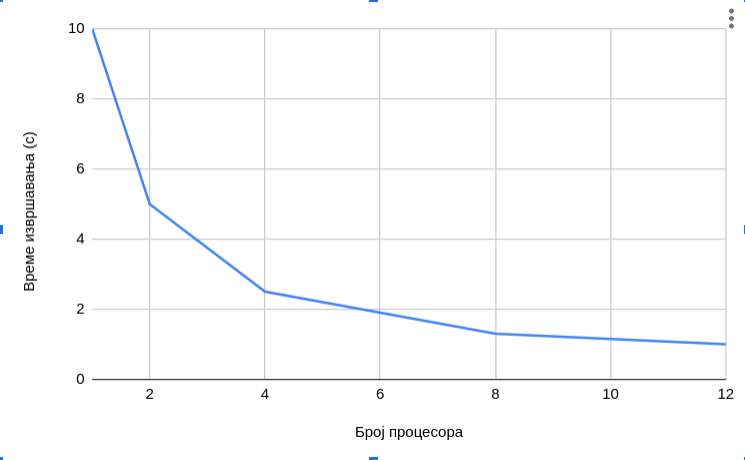
\includegraphics[scale = 0.7]{zavisnost.png}
    \caption{Резултати покретања решења са растућим бројем процесуирајућих јединица}
    \label{fig:rezultati2}
\end{figure}

На слици \ref{fig:rezultati2} приказана је брзина извршавања решења у односу на растући број процесуирајућих јединица.
Секвенцијално решење представљено је подацима о извршавању са 1 процесуирајућом јединицом.
Перформансе извршавања секвенцијалног решења су, наравно, независне од броја процесуирајућих јединица.




\pagebreak
\section{Закључак}

У овом раду, анализиран је проблем проналажења суме у бинарном стаблу.
Дат је приказ проблема и његовог секвенцијалног решења.
Потом је приказано и његово паралелно решење.
На крају, приказани су резултати који указују на линеарно убрзање доласка до решења са порастом броја процесуирајућих јединица за стабла са великим бројем чворова ($n > 10 000$).

Даљи рад на ову тему требало би узме у обзир да се са вредношћу $l$ дефинисану једначином \ref{eq:myequation} потенцијално не долази до најбољих резултата у општем случају.
То је због тога што се, са тако дефинисаном вредношћу креира укупно више задатака него што има процесуирајућих јединица.
Ово доводи до тога да, понекад, чвор на нивоу $l-1$ ни не крене да се извршава док неки од чворова нивоа $l$ не заврше своју обраду.
За неке вредности ПЈ, потенцијално би било ефикасније да се дефинише $l_{fixed}$ као $l_{fixed} = l - 1$.
Са вредношћу $l_{fixed}$ сигурни смо да сви генерисани задаци имају увек барем једну слободну процесуирајући јединицу.         % ТОДО попунити
\newpage
% 
\begin{appendices}

\section{Први додатак}
Додаци су необавезни део рада. Овде се могу убацити сирови подаци на основу којих сте, на пример, нацртали графиконе приказане у телу рада, а којих је исувише да би се приказали у самом телу рада без одвлачења пажње читаоца са шире слике утицаја добијених резултата.

\section{Други додатак}
ТОДО опционо

\end{appendices}
            % ТОДО попунити уколико су вам потребни, додаци могу бити изостављени
\newpage

\bibliographystyle{plain}
\typeout{}
\bibliography{biblist}              % ТОДО попуњавати референцама

\end{document}